% !TeX root =thesis.tex
%\subsection{Path integral approach for single channel\label{sec:pathInt}}
\label{sec:pathInt}
Randeria and the company have studied this problem with the path integral method and it is proved to be a  nice tool for the problem due to its flexibility and readiness for extension to the higher order fluctuation.  

We start with an attractive $\delta$-potential in the coordinate space.  This is not equivalent to the  reduced pairing potential as in the original BCS work.  However, the reduced paring potential only couples  particles of the opposite momentum and does not support simple form of Hubbard-Stratonovich transformation, which is essential to solve the problem in the path integral formulation.  
\begin{equation}
\hat{H}-\mu\hat{N}=\sum_{\sigma}\int{d^{d}r}c^{\dagger}_{\sigma}(\vr)\br{-\nth{2m}\nabla^{2}-\mu}c^{}_{\sigma}(\vr)-g\int{d^{d}r}c^{\dagger}_{\uparrow}(\vr)c^{\dagger}_{\downarrow}(\vr)c^{}_{\downarrow}(\vr)c^{}_{\uparrow}(\vr)
\end{equation}
 We can write down the action for the quantum partition function $\mathcal{Z}=\int{\bigD(\bar\psi,\psi)\exp\br{-S[\bar\psi,\psi]}}$
\begin{equation}\label{eq:pathInt2:actionPsi}
S[\bar\psi,\psi]=\int^{\beta}_{0}d\tau\int{d^{d}r}\mbr{\sum_{\sigma}\bar\psi_{\sigma}(\vr,\tau)\br{\partial_{\tau}-\nth{2m}\nabla^{2}-\mu}\psi_{\sigma}(\vr,\tau)-g\bar\psi_{\uparrow}(\vr,\tau)\bar\psi_{\downarrow}(\vr,\tau)\psi^{}_{\downarrow}(\vr,\tau)\psi^{}_{\uparrow}(\vr,\tau)}
\end{equation}
Notice that here fermion fields $\psi_{s}$ and $\bar\psi_{s}$ are Grassmann variables. Hence  they are not complex conjugate to each other as in the operator language because  complex conjugate is not a well-defined concept for Grassmann variables. 
We try to solve this system with Hubbard-Stratonovich transformation.   Introduce an auxiliary field (functional variable) $\Delta(\vr,\tau)$ coupled with a pair $\psi_{\uparrow}(\vr,\tau)\psi_{\downarrow}(\vr,\tau)$. %Here we follow the normal notation from path integral, $r$ is four tempo-space coordinator.  
We write down first the Gaussian integral of $\Delta$
\begin{equation}
1=\int{\bigD(\bar\Delta,\Delta)}\exp\br{-\nth{g}\int{d\tau{d}^{d}r}\bar\Delta\Delta}
\end{equation}
Note that we absorb the extra constant of integration into the measure of $\bigD(\bar\Delta,\Delta)$.
And with a shift of $\Delta(\vr,\tau)\rightarrow\Delta(\vr,\tau)-g\psi_{\uparrow}(\vr,\tau)\psi_{\downarrow}(\vr,\tau))$, we have 
\footnote{$\int{\bigD(\bar\Delta,\Delta)}\cdot1$ is only a constant factor on partition function $\mathcal{Z}$ and has no effect on real physical quantity; therefore, we can take it as 1. (This is equivalent to  divide the $\mathcal{Z}$ by a constant)}
\begin{equation}\label{eq:pathInt:expHS}
\exp\br{g\int{d\tau{}d^{d}r}\bar{\psi}_{\uparrow}\bar\psi_{\downarrow}\psi_{\downarrow}\psi_{\uparrow}}=
\int{\bigD(\bar\Delta,\Delta)}\exp\bbr{-\int{d\tau{d^{d}r}}\mbr{\nth{g}{\bar\Delta}{\Delta}-\br{\bar\Delta\psi_{\downarrow}\psi_{\uparrow}+\Delta\bar\psi_{\uparrow}\bar\psi_{\downarrow}}}}
\end{equation}
Note that  $\Delta(\vr,\tau)$ (or $\bar\Delta(\vr,\tau)$) comes from  Grassmann fields $\psi(\vr,\tau)$ (or $\bar\psi(\vr,\tau)$). Therefore, they are not related to each other as complex conjugate either.  Nevertheless, at the mean field level or only at the phase fluctuation around the mean field, $\Delta$  and $\bar\Delta$ are indeed complex conjugate.  Consequently, we will just take $\Delta$  as normal bosonic field in the following and often simply treat $\bar\Delta$ as $\Delta$'s complex conjugate in the following. Now the interaction term can be replaced.
\begin{align*}
\mathcal{Z}=&\int{}\bigD(\bar\psi,\psi)\int{\bigD(\bar\Delta,\Delta)}\\
&\;\exp\bbr{-\int{d\tau{d^{d}r}}\mbr{\sum_{\sigma}\bar\psi_{\sigma}\br{\partial_{\tau}-\nth{2m}\nabla^{2}-\mu}\psi_{\sigma}+\nth{g}{\bar\Delta}{\Delta}-\br{\bar\Delta\psi_{\downarrow}\psi_{\uparrow}+\Delta\bar\psi_{\uparrow}\bar\psi_{\downarrow}}}}
\end{align*}
At the expense of introducing an auxiliary field ($\Delta$) with contact-type coupling to the original field $\psi$, we eliminate the four-field interaction term formally.  $\Delta$ field is like a \emph{local potential} for $\psi$, although this \emph{local potential} has to be calculated from the original field self-consistently.  Nevertheless, $\Delta$ couples to a pair of fermionic field $\psi$, and thus it extracts a special degree of freedom from the $\psi$ field.  When properly selected, this degree of freedom is highly non-trivial and has macroscopic importance, which serves as ``order parameter'' for the system.  The above formula for partition function is bilinear to $\psi$, and we can rewrite it into a nicer form in Nambu spinor representation
\begin{equation}
\bar\Psi=\begin{pmatrix}\bar{\psi}_{\uparrow}&\psi_{\downarrow}\end{pmatrix}\text{,  }\qquad
\Psi=\begin{pmatrix}{\psi}_{\uparrow}\\\bar\psi_{\downarrow}\end{pmatrix}
\end{equation}
\begin{equation}\label{eq:pathInt:ZDeltaPhi}
\mathcal{Z}=\int{\bigD(\bar\Psi,\Psi)}\int{\bigD(\bar\Delta,\Delta)}\exp
	\bbr{-\int{d\tau{d^{d}r}}\mbr{\nth{g}{\bar\Delta}{\Delta}-\bar\Psi \nG\Psi}}
\end{equation}
where 
\begin{equation}\label{eq:pathInt:nG}
\nG=\begin{pmatrix}
[\hat{G}_{0}^{(p)}]^{-1}&\Delta\\\bar\Delta&[\hat{G}_{0}^{(h)}]^{-1}
\end{pmatrix}
\end{equation}
is known as the Gor'kov Green function. $[\hat{G}_{0}^{(p)}]^{-1}=-\partial_{\tau}+\nth{2m}\nabla^{2}+\mu$, and $[\hat{G}_{0}^{(h)}]^{-1}=-\partial_{\tau}-\nth{2m}\nabla^{2}-\mu$ represent the non-interacting Green functions of the particle and the hole respectively. 

Before going further, we would like to discuss one confusing point about the possible one-or-two indices for quantities such as ${G}$ or $\Delta$ in Eq. \ref{eq:pathInt:nG}.  As a matrix, such a quantity has two indices $(x,x')$ or $(p,p')$, which have no ambiguity in usage. On the other hand, there are often ambiguity when only one index $x$ or $p$ is used. In some cases, the one index means the relative value of the two indices. For example, an  interaction, $U(\vr_{1},\vr_{2})$, normally only depends on the relative coordinate, $\vr=\vr_{1}-\vr_{2}$. So $U(\vr)$ means $U(\vr_{0}+\vr,\vr_{0})$.  In other cases, especially common in the current thesis, the one index stands for its repetition.  In this case, the difference is always zero. For example, the free Green's function, $G_{0}(p)$ stands for $G_{0}(p,p')\delta({p-p'})$.  Similarly,  the order parameter, $\Delta(x)$, only couples to $\bar\psi(x)\bar\psi(x)$ (Eq. \ref{eq:pathInt:expHS}).  When used in the matrix context (Eq. \ref{eq:pathInt:nG}), it means $\Delta(x)\delta(x-x')$. Interestingly, its Fourier transformation in momentum space does not have the same properties.  In fact, it means $\Delta(p,p')=\Delta(p'-p)$.

Now action in Eq. \ref{eq:pathInt:ZDeltaPhi} is bilinear to $\Psi$; so it can be integrated out formally and the partition function then only depends on the bosonic field $\Delta$.  
\begin{equation}\label{eq:pathInt:DeltaPF}
\mathcal{Z}=\int{\bigD(\bar\Delta,\Delta)}\exp
	\bbr{-\mbr{\br{\int{d\tau{d^{d}r}}\nth{g}{\bar\Delta\Delta}}-\ln\det\nG}}
\end{equation}
And the action becomes
\begin{equation}\label{eq:pathInt:DeltaAction}
S[\bar\Delta,\Delta]=
	{\mbr{\br{\int{d\tau{d^{d}r}}\nth{g}{\bar\Delta\Delta}}-\ln\det\nG}}
\end{equation}
Note that the determinant in $\ln\det\nG$ runs through both the normal space and $2\times2$ Nambu spinor space.  The above formulas are exactly equivalent to the original partition function (action) in the fermion field $\psi$ (Eqs. \ref{eq:pathInt2:actionPsi}). It looks nice and compact. Nevertheless, $\ln\det\nG$ term is highly non-trivial and has all the many-body physics.

\section{Mean field results\label{sec:pathInt:meanfield}}
The saddle point equation of Eq. (\ref{eq:pathInt:DeltaPF}) gives the mean-field result of the system.  First we need to find the derivative of $\ln\det\nG$.  We notice the identity
\begin{equation}
\ln\det\hat{A}=\tr\ln\hat{A}
\end{equation}
and differential rule of a function like $\tr\ln$
\begin{equation}\label{eq:pathInt:diffTr}
\frac{\delta}{\delta\phi_q}\tr\ln(\nG)=\tr(\hat{\mathcal{G}}\frac{\delta}{\delta\phi_q}\nG)
\end{equation}
Using the above relations, we can write the saddle equation of Eq. (\ref{eq:pathInt:DeltaPF}) (differential with respect to $\Delta$) as
\begin{equation}
\nth{g}\bar{\Delta}(\vr,\tau)-\tr\mbr{\hat{\mathcal{G}}(\vr,\tau,\vr,\tau)\begin{pmatrix}0&1\\0&0\end{pmatrix}}=0
\end{equation}
Here this matrix is in the Nambu Spinor space.  At the  mean field level, we seek a tempo-spacial homogeneous solution of $\Delta(x)=\Delta_{0}$.  At this level,  $\Delta(p)$ becomes a $\delta$-function in the frequency-momentum space, and has non-zero elements only for two fermions with the same momentum.  (Please See the discussion in the previous section about one vs. two indices. This is not generally true, as we show it when discussing collective modes in sec. \ref{sec:collective1})
We can find the Nambu Green function from Eq. (\ref{eq:pathInt:nG}) in momentum space
\begin{equation}\label{eq:pathInt:G0}
G_{0\;p,p'}=\nth{(i\omega_n)^2-E_\vp^2}
\begin{pmatrix}
	i\omega_n+\xi_\vp&\;&-\Delta_0\\
	-\bar{\Delta}_0&\;&i\omega_n-\xi_\vp
\end{pmatrix}
\delta_{p=p'}
\equiv{}G_{0}(p)\delta_{p=p'}
\end{equation}
Here $p$ is the frequency-momentum, $p=(\omega_{n},\vp)$, and $\omega_n$ is the Matsubara frequency of Fermions.  $\xi_{\vk}=\epsilon_{\vk}-\mu$, $\epsilon_{\vk}=\vk^{2}/2m$,  $E_\vp=\sqrt{\xi_\vp^2+\abs{\Delta_0}^2}$.  And the saddle point equation can be rewritten as 
\begin{equation}
\nth{g}\bar{\Delta}_0=\frac{T}{L^d}\sum_{\vp,n}\frac{\bar\Delta_0}{\omega_n^2+E_\vp^2}
\end{equation}
The summation of Matsubara frequency can be evaluated and we find 
\begin{equation}
\nth{g}=\nth{L^d}\sum_{\vp}\frac{1-2n_f(E_p)}{2E_p}=\nth{L^d}\sum_{\vp}\frac{\tanh{(E_p/2T)}}{2E_p}
\label{eq:pathInt:gap}
\end{equation}
where $n_f(\epsilon)$ is the fermi distribution function.  This is exactly the famous gap equation obtained from other methods as well.  On the other hand, $\nG$ in Eq. (\ref{eq:pathInt:nG})  is the inverse of the  fermion-fermion correlation of $\Psi$.  In the mean field, $G_{0}$ as Eq. (\ref{eq:pathInt:G0}) can be diagonalized in the momentum space with a canonical (Bogoliubov) transformation.  We can make an analytic continuation of $i\omega_{n}\rightarrow\omega+0^{+}$.  Eq. (\ref{eq:pathInt:G0})  then has poles ($\pm{}E_{p}$) where  $\omega^2-E_\vp^2=0$,  which determine  the spectrum of fermionic excitation.  

Summand in Eq. \ref{eq:pathInt:gap} does not decreases fast enough in 3D and the summation does not converges.  This is because our assumption of contact interaction breaks down for the scale smaller than real potential range $r_{c}$, i.e., the summation of momentum is capped at some high momentum $\Lambda$ related to $1/r_{c}$.  Notice that in 3D, we have a similar relation that connect the bare potential $g$ to a more physically observable quantity, the s-wave scattering length $a_{s}$
\begin{equation}\label{eq:pathInt:as}
\frac{m\mathcal{V}_{0}}{4\pi{}a_{s}}=-\nth{g}+\sum_{k<\Lambda}\nth{2\epsilon_{\vk}}
\end{equation}
Here $\mathcal{V}_{0}$ is the total volume.  We can renormalize Eq. \ref{eq:pathInt:gap} with this relation
\begin{equation}\label{eq:pathInt:gapRenormalized}
-\frac{m\mathcal{V}_{0}}{4\pi{}a_{s}}=\sum_{\vk}\mbr{\frac{\tanh{(E_k/2T)}}{2E_k}-\nth{2\epsilon_{\vk}}}
\end{equation}
Now the gap equation has proper decay in high momentum and no artificial cutoff is necessary.  There are two unknown parameters, $\mu$ and $\Delta$,  in the equation.  We need another equation in order to pin them down. To compliment the gap equation, we can introduce the number equation, $N=-\partial\Omega/\partial\mu$. At the saddle point, the thermodynamic potential is $\Omega_{0}=S[\Delta_{0}]/\beta$, and we have number equation
\begin{equation*}
N=-\nth{\beta}\tr\br{{G_{0}\pdiff{G_{0}^{-1}}{\mu}}}
\end{equation*}
Similarly the summation (due to the trace) over the Mastubara frequency can be evaluated and we have the number equation
\begin{equation}
N=\nth{L^{d}}\sum_{\vk}\mbr{1-\frac{\epsilon_{\vk}}{E_{\vk}}\tanh{(\frac{E_{\vk}}{2T})}}
\end{equation}
This equation has no divergence at high momentum.  The number equation  and the renormalized gap equation Eq. \ref{eq:pathInt:gapRenormalized} compose the implicit equations for two unknown parameters, gap $\Delta$ and chemical potential $\mu$.  It is not hard to find the zero temperature analytic result at both ends.  At the BCS end ($1/k_{F}a_{s}\rightarrow-\infty$), we obtain $\mu\approx{}E_{F}$ and $\Delta\propto\exp(-\pi/2k_{F}\abs{a_{s}})$; at the BEC end ($1/k_{F}a_{s}\rightarrow+\infty$),  $\mu=-\hbar^{2}/2ma_{s}^{2}$, i.e. half of the binding energy of a molecule, while $\Delta\propto{}n^{1/2}a_{s}^{-1/2}$ no longer has  much physical significance.  In the more general crossover region, these two equations need to be solved numerically.  They have no singularity in the whole region, which indicates it is a crossover instead of any simple phase transition.  Please see Fig. \ref{fig:pathInt:meanField} for detail. 
\begin{figure}[htbp]
\begin{center}
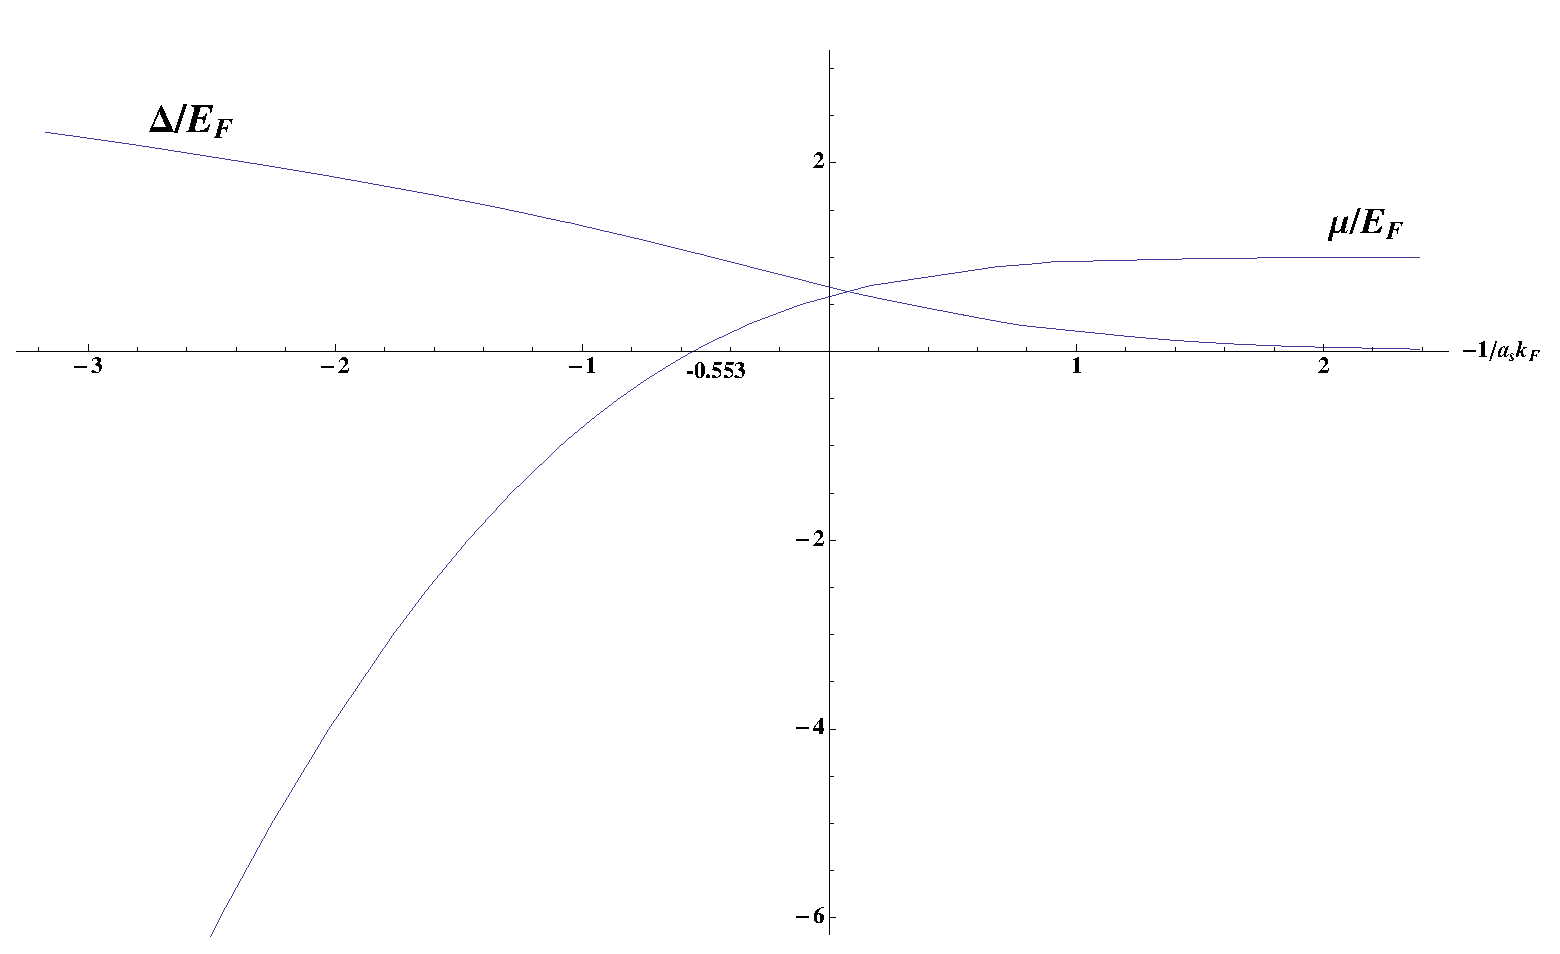
\includegraphics[width=0.8\textwidth]{SingleChannelCrossoverMuDelta}
\caption{The chemical potential $\mu$ and gap $\Delta$ in the mean field level over crossover} 
\label{fig:pathInt:meanField}
{\small All energy-like quantities ($\mu$, $\Delta$) are rescaled with the Fermi energy $E_{F}$ and the s-wave scattering length $a_{s}$ is rescaled with $1/k_{F}$.  }
\end{center}
\end{figure}



\section{Gaussian fluctuation and collective modes}\label{sec:collective1}
We can expand the partition function Eq. (\ref{eq:pathInt:DeltaPF}) around the mean-field value, $\Delta(\vr,\tau)=\Delta_{0}+\theta(\vr,\tau)$. The linear order of the  expansion is zero because $\Delta_{0}$ is the saddle point.  The next order gives us the bilinear terms on $\theta$, i.e., correlation of bosonic fields $\Delta$ (four-fermion correlation).  Note that here the Hamiltonian only has an contact-type potential, therefore it cannot cover the situation of a charged system where long-range Columnb interaction cannot be neglected.  We limit ourselves to the neutual case.  Nevertheless, it is conceivable that a more realistic short-range potential only renormalizes some parameters in the following calculation while leaves the qualitative result unmodified.  

Notice that we can expand the second term in Eq. \ref{eq:pathInt:DeltaPF} for $\hat{G}{}^{-1}=\hat{G}_{0}^{-1}+\hat{K}$
\begin{equation}\label{eq:pathInt:expand}
\tr\ln \hat{G}^{-1}=\tr\ln\hat{G_{0}}^{-1}+\tr(\hat{G_{0}}\hat{K})-\nth{2}\tr(\hat{G_{0}}\hat{K}\hat{G_{0}}\hat{K})+\cdots
\end{equation}
In our case,
\begin{equation}
\hat{K}=\begin{pmatrix}
0&\theta\\
\theta^{*}&0
\end{pmatrix}
\end{equation}
Here the linear terms of $\hat{K}$ or $\theta$ ($\theta^{*}$) are zero as the saddle point condition.  So to the second order, the action is 
\begin{equation}\label{eq:pathInt:DeltaActionGaussian}
S[\Delta_{0},\theta,\theta^{*}]=S[\Delta_{0}]+
	\nth{2g}\tr(\hat{K}\hat{K})+\nth{2}\tr(\hat{G_{0}}\hat{K}\hat{G_{0}}\hat{K})
\end{equation}
Write the last term into the momentum representation
\begin{equation}
\tr(\hat{G_{0}}\hat{K}\hat{G_{0}}\hat{K})=\sum_{q,p}\Tr\br{G_{0}({p})K_{q}G_{0}{}({p-q})K_{-q}}
\end{equation}
Notice that the second ``$\Tr$'' and following ``$\Tr$'' in this section only runs in Nambu spinor space and $q={(\vq,q_{l})}$, $p=(\vp,p_{n})$ are all four momentum, where $q_{l}$ is the bosonic Matsubara frequency while $p_{n}$ is the fermionic Matsubara frequency.
\begin{equation}
K_{p_{0},p_{0}+q}=K_{q}=\begin{pmatrix}
0&\theta_{q}\\
\theta^{*}_{-q}&0
\end{pmatrix}
\end{equation}
And we remember that $G_{0}(p)=G_{0}{}_{p,p}$
If we introduce  a new vector 
\begin{equation}
\theta{(q)}=\begin{pmatrix}\theta_{q}\\\theta^{*}_{-q}\end{pmatrix}\qquad
\theta^{\dg}{(q)}=\begin{pmatrix}\theta^{*}_{q}&\theta_{-q}\end{pmatrix}
\end{equation}
the action can be rewritten into a more compact form
\begin{equation}
S[\Delta_{0},\theta,\theta^{*}]=S[\Delta_{0}]+\nth{2}\sum_{q}\mbr{\theta^{\dg}(q)\mathbf{M}(q)\theta(q)}
\end{equation}
Notice that we can always choose a real $\Delta_{0}$ and therefore $G_{0}{\ _{12}}(p)=G_{0}{\ _{21}}(p)$, we have 
\begin{equation}
\mathbf{M}_{q,q}=\mathbf{M}(q)=
\begin{pmatrix}
\nth{g}+\sum_{p}G_{0}{\ }_{11}(p)G_{0}{\ }_{22}(p-q)&\sum_{p}G_{0}{\ }_{12}(p)G_{0}{\ }_{12}(p-q)\\
\sum_{p}G_{0}{\ }_{12}(p)G_{0}{\ }_{12}(p-q)&\nth{g}+\sum_{p}G_{0}{\ }_{11}(p-q)G_{0}{\ }_{22}(p)
\end{pmatrix}
\end{equation}
The summation over  the (fermionic) Matsubara frequency of $p_{n}$ can be carried out at zero temperature
\footnote{\label{foot:intro:sum}The summation of the Matsubara frequency of a function $h(i\omega_{n})$ is carried out by the normal trick.  We  multiply $h(z)$ with the Fermi distribution function $n_{F}(z)$,  the summation is the sum of residuals at the imaginary axis of $n_{F}(z)$.  The contour can be deform into a contour over the rest of singular points of $h(z)$. We just need to find the residuals of the total function $h(z)n_{F}(z)$ over those singular points to find the Matsubara summation.   However, due to zero temperature, the  $n_{F}(z)$ is only nonzero at the negative singular points of $h(z)$, $-E_{\vk}$ in this case.  (The other singular point $E_{\vk}$ gives $n_{F}(E_{\vk})=0$ for zero temperature.)}
\begin{equation}
\begin{split}
M_{11}(q)&=M_{22}(-q)\\
	&=\nth{g}+\sum_{\vp{,}p_{n}}G_{0}{\ }_{11}(p)G_{0}{\ }_{22}(p-q)\\
	&=\nth{g}+\sum_{\vp}\br{\frac{u^{2}u'^{2}}{iq_{l}-E-E'}-\frac{v^{2}v'^{2}}{iq_{l}+E+E'}}
\end{split}
\end{equation}
\begin{equation}
\begin{split}
M_{12}(q)&=M_{21}(q)\\
	&=\sum_{\vp{,}p_{n}}G_{0}{\ }_{12}(p)G_{0}{\ }_{12}(p-q)\\
	&=\sum_{\vp}uvu'v'\br{\nth{iq_{l}+E+E'}-\nth{iq_{l}-E-E'}}
\end{split}
\end{equation}
where $u=u_{\vp}$, $v=v_{\vp}$, $E=E_{\vp}$ and $u'=u_{\vp-\vq}$, $v'=v_{\vk-\vq}$, $E'=E_{\vk-\vq}$.  $u$, $v$, $E$ are as defined usually in BCS literature. 
\begin{equation}
v_{\vk}^{2}=1-u_{\vk}^{2}=\nth{2}\br{1-\frac{\xi_{\vk}}{E_{\vk}}}
\end{equation}
 The $G^{(M)}=\mathbf{M}^{-1}$ is the correlation function of $\theta$ (or $\Delta$) and its poles give the spectrum of collective modes as every  $\theta_{q}$ (or $\Delta_{q}$) involves many fermions moving in a coherent manner.  So the spectrum of collective modes can be determined by finding poles of $G^{(M)}$, $\det{M(\omega,\vq)}=0$ after we analytically continue for the frequency $iq_{l}\rightarrow\omega+i0^{+}$.  
 
For low energy modes, where $\omega,\,\abs{\vq}^{2}$ both are much smaller than $\min\bbr{E_{\vk}}=\Delta_{0}$, we can expand $M$ with $\omega$ and $\vq$.  The lowest order has the form $\omega\approx{}c\,q$, which suggests a sound wave as expected for any Goldstone mode.  At BCS side, $c=v_{F}/\sqrt{3}$, where $v_{F}$ is Fermi velocity.  This coincides with the famous Anderson-Bogoliubov mode.  At the BEC side, we get $c^{2}=\Delta^{2}/8m\abs{\mu}=v_{F}^{2}(k_{F}a_{s})/3\pi=4\pi{}n_{B}a_{B}/m_{B}$, which fits the low momentum part of Bogoliubov spectrum.  Here $m_{B}=2m$ is the molecule mass, $n_{B}=n/2$ is the molecule density and $a_{B}=2a_{s}$ is the inferred  interaction between molecules.  This value differs from the result of more accurate calculation from few-body, $a_{B}=0.6a_{s}$, which indicates the possible deficiency of the theory. 


\section{An alternative method to invert the Green's function\label{sec:diagonalizeGreen1}}
In the above section, we inverted the  Gor'kov green function matrix Eqs. (\ref{eq:pathInt:nG}, \ref{eq:pathInt:G0}) directly and it is not hard to do as a $2\times2$ matrix in the  momentum space.   Alternatively, we can use a different approach which proves to be more convenient in the two-channel problem.  First, we diagonalize $\nG$ with a unitary transformation $T$, in the momentum space
\begin{equation}
\nG=\mtrx{i\omega_{n}-\xi_{k}&\Delta\\\bar\Delta&i\omega_{n}+\xi_{k}}=T^{\dg}BT
\end{equation}
It is easy to show that such $T$ and $B$ satisfying above equation are
\begin{equation}
T=\mtrx{u_{k}&v_{k}\\-v_{k}^{*}&u_{k}}\qquad{}B=\mtrx{i\omega_{n}+E_{k}&0\\0&i\omega_{n}-E_{k}}
\end{equation}
where $u_{k}^{2}(v_{k}^{2})=\nth{2}(1\pm\xi_{k}/E_{k})$ and $E_{k}=\sqrt{\xi^{2}_{\vk}+\Delta^{2}}$ are conventionally defined quantities in the BCS theory.   Actually, this transformation is nothing but the Bogoliubov canonical transformation, and $B$ matrix simply describes spectrum of fermionic quasi-particles.  Now it is easy to invert $\nG$
\begin{equation}
G=T^{\dg}B^{-1}T
\end{equation}
Green's function $G$ takes a more conventional form $A/(i\omega_{n}\pm{}E_{k})$ without any dependency on frequency in nominator as Eq. (\ref{eq:pathInt:G0}). Matsubara frequency summation over $G_{0}(k)$ in the mean-field and $G_{0}(k)G_{0}(k+q)$ in the Gaussian order are then fairly straight-forward as in text-book.  
